\section{数列的基本概念}

\begin{theorem}
    按照一定次序排列的一列数称为数列 (Sequence).

    数列中的每一个数都叫做这个数列的项 (Term)．记作 $\{a_n\}$，其中 $a_n$ 称为数列的通项。
\end{theorem}

\subsection{数列的通项公式}

\begin{definition}
    数列 $\{a_n\}$ 的通项公式是一个函数 $f(n)$，使得对于每个正整数 $n$，都有 $a_n = f(n)$。

    数列实际上就是一个函数中，只取了正整数的部分，这些离散的点组合起来，称为数列。

    \begin{center}
        \begin{tikzpicture}[scale=0.9]
            % 函数和数列的表示
            \draw[->] (-0.5,0) -- (7,0) node[right] {$x$};
            \draw[->] (0,-0.5) -- (0,5) node[above] {$y$};

            % 连续函数曲线
            \draw[blue, thick, domain=0.2:3, smooth] plot (\x, {0.5*\x*\x})
            node[right] {$f(x) = \frac{x^2}{2}$};

            % 数列点
            \foreach \x in {1,2,3} {
                    \fill[red] (\x, {0.5*\x*\x}) circle (3pt);
                    \draw[dashed] (\x, 0) -- (\x, {0.5*\x*\x});
                    \draw[dashed] (0, {0.5*\x*\x}) -- (\x, {0.5*\x*\x});
                }

            % 注释
            \node[red] at (4, 3) {数列 $\{a_n\}$ 是函数在正整数上的取值};

            % 标记示例点
            \node[below] at (3, 0) {$n=3$};
            \node[left] at (0, {0.5*3*3}) {$a_3=4.5$};
        \end{tikzpicture}
    \end{center}
\end{definition}

\begin{example}
    数列 $1, \frac{1}{2}, \frac{1}{3}, \frac{1}{4}, \dots$ 的通项公式可以表示为 $a_n = \frac{1}{n}$。
\end{example}

\v{2em}

\begin{problem}
数列 $1,4,9,16,25,...$ 的通项公式如何表示？
\end{problem}

\v{2em}

\subsubsection{数列的正整数性}

\begin{theorem}
    数列中的 $a_n$ 一定是满足 $n \in \mathbf{N}^*$ 的条件，即 $n$ 是正整数。
\end{theorem}

\begin{example}
    求数列 $a_n = n + \frac{5}{n}$ 的最小项是第几项？
\end{example}

\v{6em}

\subsection{数列的前 $n$ 项和}

\begin{definition}
    数列 $\{a_n\}$ 的前 $n$ 项和记作 $S_n = a_1 + a_2 + \cdots + a_n$，其中 $n$ 是正整数。
\end{definition}

\begin{theorem}
    数列 $\{a_n\}$ 的前 $n$ 项和 $S_n$ 的通项公式可以使用 Sum 符号表示。为：$S_n = \sum_{k=1}^{n} a_k$。
\end{theorem}

\begin{problem}
数列 $1,4,9,16,25,...$ 的前 $n$ 项和是多少？
\end{problem}

\begin{theorem}[平方和公式和立方和公式]
    $$ 1^2 + 2^2 + 3^2 + \dots + n^2 $$
    其求和公式为：
    $$ \sum_{i=1}^{n} i^2 = \frac{n(n+1)(2n+1)}{6} $$

    $$ 1^3 + 2^3 + 3^3 + \dots + n^3 $$
    其求和公式为：
    $$ \sum_{i=1}^{n} i^3 = \left[ \frac{n(n+1)}{2} \right]^2 $$
\end{theorem}

\begin{proof}
    我们使用草垛法证明。对于不同的 $n \times n$ 的正方形，可以取：
    \begin{center}
        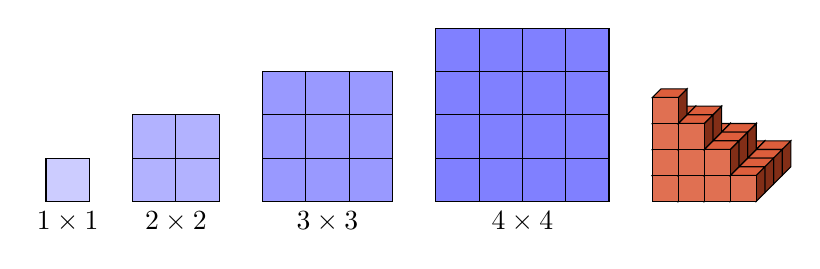
\begin{tikzpicture}[scale=0.55]
            \begin{scope}[shift={(-4,0)}]
                \draw[fill=blue!20] (0,0) rectangle (1,1);
                \draw[thin] (0,0) grid (1,1);

                \draw[fill=blue!30] (2,0) rectangle (4,2);
                \draw[thin] (2,0) grid (4,2);

                \draw[fill=blue!40] (5,0) rectangle (8,3);
                \draw[thin] (5,0) grid (8,3);

                \draw[fill=blue!50] (9,0) rectangle (13,4);
                \draw[thin] (9,0) grid (13,4);

                \begin{scope}[shift={(14,0)},
                        x = {(0.6cm, 0cm)},
                        y = {(0.2cm, 0.2cm)},
                        z = {(0cm, 0.6cm)}]

                    \colorlet{cube_front}{red!40!brown!80}
                    \colorlet{cube_right}{red!40!brown!60!black}
                    \colorlet{cube_top}{red!40!brown!90!white}

                    \foreach \z in {0, 1, 2, 3} {
                            \pgfmathtruncatemacro{\layersize}{3 - \z}
                            \foreach \y in {\layersize, ..., 0} {
                                    \foreach \x in {0, ..., \layersize} {
                                            \coordinate (pos) at (\x, \y, \z);

                                            \fill[cube_right, draw=black, thin] (pos) ++(1,0,0) -- ++(0,1,0) -- ++(0,0,1) -- ++(0,-1,0) -- cycle;
                                            \fill[cube_top, draw=black, thin] (pos) ++(0,0,1) -- ++(1,0,0) -- ++(0,1,0) -- ++(-1,0,0) -- cycle;
                                            \fill[cube_front, draw=black, thin] (pos) -- ++(1,0,0) -- ++(0,0,1) -- ++(-1,0,0) -- cycle;
                                        }
                                }
                        }
                \end{scope}

                \node[below] at (0.5,0) {$1\times1$};
                \node[below] at (3,0) {$2\times2$};
                \node[below] at (6.5,0) {$3\times3$};
                \node[below] at (11,0) {$4\times4$};
            \end{scope}
        \end{tikzpicture}
    \end{center}
    我们把它复制成三份，则有 $3(1^2+2^2+3^2+\cdots+n^2)$.

    \begin{figure}[H]
        \centering
        \begin{minipage}[c]{0.45\textwidth}
            \centering
            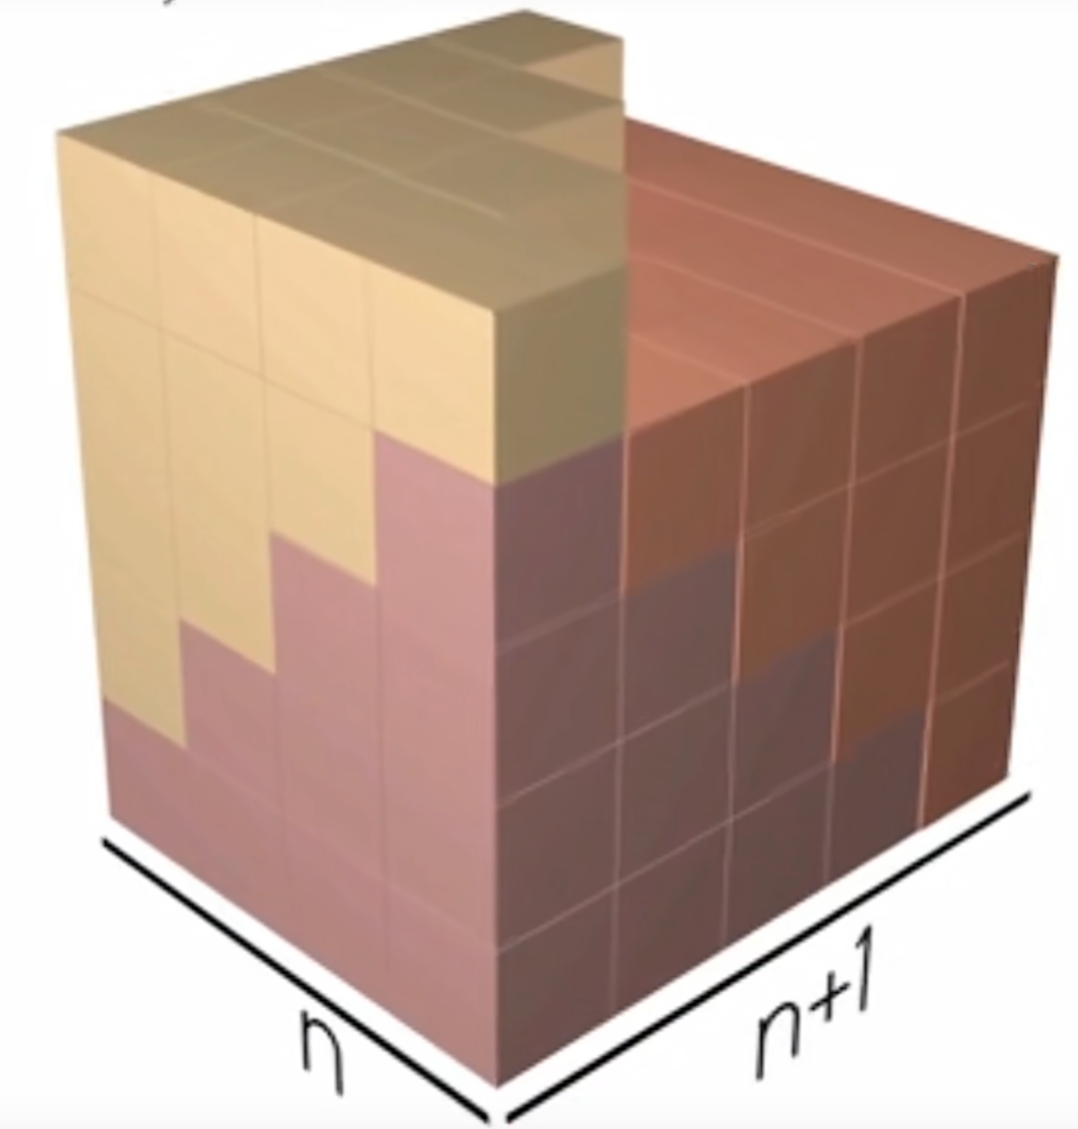
\includegraphics[width=0.4\textwidth]{chapters/数列/images/数列基本定义/img-20250805232353.png}
            \caption*{复制成三份}
        \end{minipage}
        \hfill
        \begin{minipage}[c]{0.45\textwidth}
            \centering
            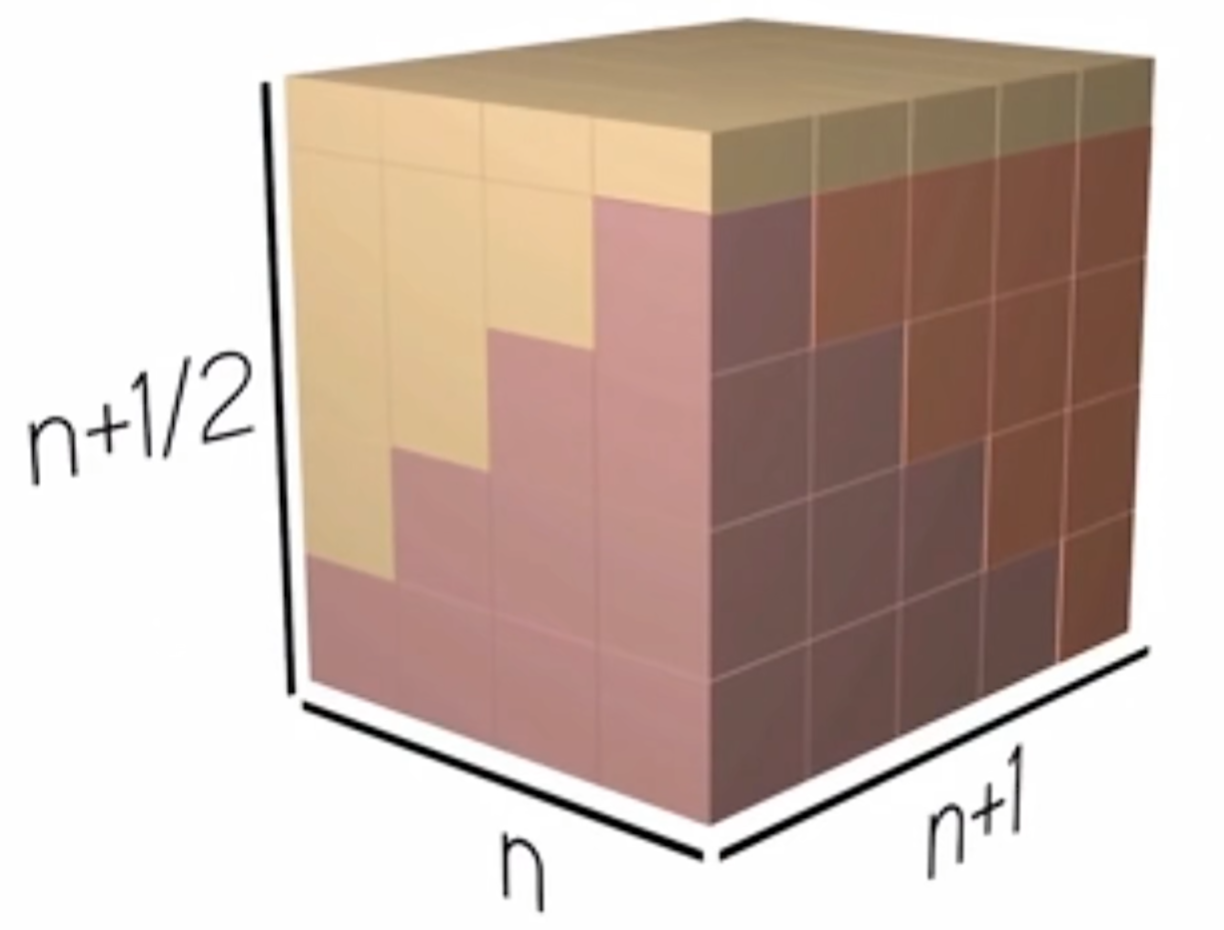
\includegraphics[width=0.5\textwidth]{chapters/数列/images/数列基本定义/img-20250805232710.png}
            \caption*{补全成立体形状}
        \end{minipage}
    \end{figure}

    再把顶层的一半补全到剩下的位置，就会有高为 $n+\frac{1}{2}$.
    乘起来除以 $3$ 即可得到正确结果。
\end{proof}

\begin{tips}
    此处，感谢 \href{https://www.bilibili.com/video/BV1wR4y1a7yh}{https://www.bilibili.com/video/BV1wR4y1a7yh} 的视频讲解。
\end{tips}

\subsection{$S_n$ 与 $a_n$ 的关系}

\begin{theorem}
    对于任意数列 $\{a_n\}$，其前 $n$ 项和为 $S_n = a_1 + a_2 + \dots + a_n$。
    其通项 $a_n$ 与前 $n$ 项和 $S_n$ 存在如下关系：
    $$
        a_n =
        \begin{cases}
            S_1           & n=1      \\
            S_n - S_{n-1} & n \geq 2
        \end{cases}
    $$
    此关系对任意数列都成立，是求通项公式的重要方法。使用后务必检验 $n=1$ 是否符合 $n \geq 2$ 的表达式。
\end{theorem}

\begin{example}
    已知数列 $\{a_n\}$ 的前 $n$ 项和 $S_n = 2n^2 - n$，则其通项公式 $a_n$ 为 \underline{\qquad}
\end{example}

\v{8em}

\begin{example}
    设数列 $\{a_n\}$ 的前 $n$ 项和为 $S_n = n^2 + 3n + 1$。求数列的通项公式 $a_n$。
\end{example}

\v{8em}

\begin{warning}
    数列中一旦一个式子里同时出现了 $a_n$ 和 $S_n$，都是要把 $S_n$ 消掉的！这样才能完整地得到 $a_n$ 的关系！

    方法是令 $n$ = $n-1$
\end{warning}

\begin{example}
    （2023·甲卷·理 17）设 $S_n$ 为数列 $\left\{a_n\right\}$ 的前 $n$ 项和，已知 $a_2=1,2 S_n=n a_n$ ．
    \begin{enumerate}
        \item 求 $\left\{a_n\right\}$ 的通项公式；
    \end{enumerate}
\end{example}

\v{6em}

\begin{example}
    （2021·浙江·20）已知数列 $\left\{a_n\right\}$ 的前 $n$ 项和为 $S_n, a_1=-\frac{9}{4}$ ，且 $4 S_{n+1}=3 S_n-91$ ．
    \begin{enumerate}
        \item （1）求数列 $\left\{a_n\right\}$ 的通项；
    \end{enumerate}
\end{example}

\v{6em}

\subsection{数列的单调性}

\begin{theorem}
    严格增数列和严格减数列应该分别满足：

    \begin{itemize}
        \item 严格增数列：对于任意的正整数 $n$，都有 $a_n < a_{n+1}$。
        \item 严格减数列：对于任意的正整数 $n$，都有 $a_n > a_{n+1}$。
    \end{itemize}
\end{theorem}

\begin{example}
    已知数列 $\left\{a_n\right\}$ 的通项公式为 $a_n=\frac{k-n}{3^n}$ ，若 $\left\{a_n\right\}$ 是递增数列，则 $k$ 的取值范围为 （\qquad）
    \begin{tasks}(4)
        \task $(-\infty, 1)$
        \task $(1,+\infty)$
        \task $\left(-\infty, \frac{1}{2}\right)$
        \task $\left(\frac{1}{2},+\infty\right)$
    \end{tasks}
\end{example}

\v{12em}

\begin{example}
    已知数列 $\left\{a_n\right\}$ 是严格增数列且 $a_n=n^2+k n+2$（ $n$ 为正整数），则实数 $k$ 的取值范围为 \underline{\qquad}.
\end{example}

\begin{solution}
    因为数列 $\left\{a_n\right\}$ 是严格增数列，则对任意的 $n \in \mathbf{N}^*, a_{n+1}>a_n$

    即 $(n+1)^2+k(n+1)+2>n^2+k n+2$ ，可得 $k>-2 n-1$

    显然数列 $\{-2 n-1\}$ 为递减数列，故 $k>(-2 n-1)_{\max }=-3$

    因此，实数 $k$ 的取值范围是 $(-3,+\infty)$.
\end{solution}

\v{12em}

\begin{example}
    已知数列 $\left\{a_n\right\}$ 的通项公式为 $a_n=\frac{3^n-1}{3^n}$ ，前 $n$ 项和为 $S_n$ ，则下列结论正确的是 （\qquad）（\textcolor{red}{D 留到之后做}）
    \begin{tasks}(4)
        \task $a_1=\frac{2}{3}$
        \task $\left\{a_n\right\}$ 是递减数列
        \task $a_n \geq \frac{2}{3}$
        \task $S_n>n-\frac{1}{2}$
    \end{tasks}
\end{example}

\v{12em}

\begin{example}
    已知数列 $\left\{a_n\right\}$ 的前 $n$ 项和 $S_n=9 n-n^2$ ，则下列说法正确的是 （\qquad）
    \begin{tasks}(4)
        \task $S_n$ 的最大值为 20
        \task $a_1, a_7, a_4$ 成等比数列
        \task 数列 $\left\{\frac{S_n}{n}\right\}$ 是递减数列
        \task 数列 $\left\{\frac{a_n}{n}\right\}$ 是递增数列
    \end{tasks}
\end{example}

\v{12em}

\begin{example}
    已知数列 $\left\{a_n\right\}$ 不是递增数列，且 $a_n=\left\{\begin{array}{l}3, n=1 \\ 2 k n-k+1, n \geq 2\end{array}\right.$ ，则 $k$ 的取值范围为  \underline{\qquad}.
\end{example}

\begin{tips}
    请分为 $k > 0$ 和 $k < 0$ 两种情况来做。
\end{tips}

\v{10em}

\begin{example}
    已知数列 $\left\{a_n\right\}$ 满足 $a_n=\left\{\begin{array}{l}(1-3 a) n+15 a, n \leq 4 \\ 4 a^{n-3}+4, n \geq 5\end{array}\right.$ ，若 $\forall n \in \mathbf{N}^*, a_{n+1}<a_n$ 恒成立，则实数 $a$ 的取值范围是 （\qquad）
    \begin{tasks}(4)
        \task $\left(0, \frac{3}{4}\right)$
        \task $\left(\frac{1}{3},+\infty\right)$
        \task $\left(\frac{1}{3}, \frac{3}{4}\right)$
        \task $\left(\frac{1}{3}, \frac{3}{4}\right]$
    \end{tasks}
\end{example}

\begin{tips}
    回顾必修一单调性的知识即可。
\end{tips}

\v{10em}

\begin{example}
    已知函数 $f(x)=\left\{\begin{array}{c}x^2+a x+5, x \leq 1 \\ -\frac{a}{x}, x>1\end{array}\right.$ 是 $\mathbf{R}$ 上的减函数，则实数 $a$ 的取值范围是 （\qquad）
    \begin{tasks}(4)
        \task $-3 \leq a \leq-2$
        \task $-3 \leq a \leq 0$
        \task $a \leq-2$
        \task $a<0$
    \end{tasks}
\end{example}

\v{10em}

\begin{example}
    已知函数 $f(x)=\left\{\begin{array}{l}-x^2-a x-5, x \leq 1 \\ \frac{a}{x}, x>1\end{array}\right.$ 是 R 上的增函数，则 $a$ 的取值范围是 （\qquad）
    \begin{tasks}(4)
        \task $-3 \leq a \leq-2$
        \task $a \leq-2$
        \task $-3 \leq a \leq 0$
        \task $a \leq 0$
    \end{tasks}
\end{example}

\v{10em}

\subsection{周期数列}

\begin{theorem}
    如果数列 $\{a_n\}$ 存在正整数 $p$ 使得对于任意的正整数 $n$，都有 $a_{n+p} = a_n$，则称 $\{a_n\}$ 为周期数列，$p$ 称为周期。
\end{theorem}

\begin{tips}
    并不是所有的数列都能简单地看出周期是多少。

    在处理周期数列时，可以通过观察数列的前几项来猜测周期。
\end{tips}

\begin{example}
    数列 $\left\{a_n\right\}$ 满足 $a_{n+1}=\left\{\begin{array}{l}2 a_n, 0 \leq a_n \leq 1 \\ a_n-1,\left(a_n>1\right)\end{array}\right.$ ，且 $a_1=\frac{6}{7}$ ，则 $a_{2017}=$ \underline{\qquad}.
\end{example}

\v{12em}

\begin{example}
    在数列 $\left\{a_n\right\}$ 中，已知 $a_1=6, ~ a_2=3, ~ a_{n+1}=a_{n+2}+a_n$ ，则 $a_{2025}$= （\qquad）
    \begin{tasks}(4)
        \task 3
        \task -3
        \task 6
        \task -6
    \end{tasks}
\end{example}

\begin{solution}
    数列 $\left\{a_n\right\}$ 中，由 $a_{n+1}=a_{n+2}+a_n$ ，得

    $~ a_{n+2}=a_{n+3}+a_{n+1}$ ，所以 $a_{n+3}=-a_n$ ，所以 $a_{n+6}=-a_{n+3}=a_n$

    因此数列 $\left\{a_n\right\}$ 是周期数列，周期为 6 ，所以 $a_{2025}=a_{337 \times 6+3}=a_3=-3$
\end{solution}

\v{12em}

\begin{example}
    已知数列 $\left\{a_n\right\}$ 满足 $a_1=1, a_{n+1}=2-\frac{4}{a_n}$ ，则 $\left\{a_n\right\}$ 的前 2025 项和为 （\qquad）
    \begin{tasks}(4)
        \task 2024
        \task 2025
        \task 2026
        \task 2027
    \end{tasks}
\end{example}

\v{12em}

\subsection{数列求和}

\begin{example}
    （2020·浙江·11）已知数列 $\left\{a_n\right\}$ 满足 $a_n=\frac{n(n+1)}{2}$ ，则 $S_3=$ \underline{$\quad$} ．
\end{example}

\vspace{6em}

\begin{example}
    （2019·上海·8）已知数列 $\left\{a_n\right\}$ 前 $n$ 项和为 $S_n$ ，且满足 $S_n+a_n=2$ ，则 $S_5=$ \underline{$\quad$} ．
\end{example}

\vspace{6em}
